
\let\negmedspace\undefined
\let\negthickspace\undefined
\documentclass[journal]{IEEEtran}
\usepackage[a5paper, margin=10mm, onecolumn]{geometry}
%\usepackage{lmodern} % Ensure lmodern is loaded for pdflatex
\usepackage{tfrupee} % Include tfrupee package

\setlength{\headheight}{1cm} % Set the height of the header box
\setlength{\headsep}{0mm}     % Set the distance between the header box and the top of the text

\usepackage{gvv-book}
\usepackage{gvv}
\usepackage{cite}
\usepackage{amsmath,amssymb,amsfonts,amsthm}
\usepackage{algorithmic}
\usepackage{graphicx}
\usepackage{textcomp}
\usepackage{xcolor}
\usepackage{txfonts}
\usepackage{listings}
\usepackage{enumitem}
\usepackage{mathtools}
\usepackage{gensymb}
\usepackage{comment}
\usepackage[breaklinks=true]{hyperref}
\usepackage{tkz-euclide} 
\usepackage{listings}
% \usepackage{gvv}                                        
\def\inputGnumericTable{}                                 
\usepackage[latin1]{inputenc}                                
\usepackage{color}                                            
\usepackage{array}                                            
\usepackage{longtable}                                       
\usepackage{calc}                                             
\usepackage{multirow}                                         
\usepackage{hhline}                                           
\usepackage{ifthen}                                           
\usepackage{lscape}
\begin{document}

\bibliographystyle{IEEEtran}
\vspace{3cm}

\title{NCERT-10.4.4.1.2}
\author{EE24BTECH11023 - RASAGNA}

% \maketitle
% \newpage
% \bigskip
{\let\newpage\relax\maketitle}

\renewcommand{\thefigure}{\theenumi}
\renewcommand{\thetable}{\theenumi}
\setlength{\intextsep}{10pt} % Space between text and floats


\numberwithin{equation}{enumi}
\numberwithin{figure}{enumi}
\renewcommand{\thetable}{\theenumi}
\textbf{Question:}
Find the nature of the roots of the following quadratic equation. If the real roots exist,find them:
\begin{align*}
    3x^2-4{\sqrt{3}}x+4=0
\end{align*}
\textbf{Theoritical Solution:}
The standard quadratic equation is:
\begin{align}
    ax^2 + bx + c = 0
\end{align}
Here, \( a = 3, b = -4{\sqrt{3}}, c = 4 \).
Computing the value of determinant,
\begin{align}
    \triangle =b^2-4ac
\end{align}
\begin{align}
    \triangle =(-4{\sqrt{3}})^2-4(3)(4)
\end{align}
\begin{align}
    \therefore \triangle =0
\end{align}
$\therefore$ The given equation has two equal and real roots.\\
The roots are given by:
\begin{align}
    x = \frac{-b \pm \sqrt{b^2 - 4ac}}{2a}
\end{align}
Substitute the values of \( a, b, \) and \( c \):
\begin{align}
   & x = \frac{-(-4{\sqrt{3}}) \pm \sqrt{(-4{\sqrt{3}})^2 - 4(3)(4)}}{2(3)} \\
   & = \frac{2}{\sqrt{3}}
\end{align}
Thus, the roots of the equation are:
\begin{align}
x_1=x_2=\frac{2}{\sqrt{3}}
\end{align}
\textbf{ Solution using Matrix Approach by finding eigen values}\\
\textbf{Matrix-Based Method}\\
For a polynomial equation of the form:
\begin{align}
    x^n + b_{n-1}x^{n-1} + \cdots + b_2x^2 + b_1x + b_0 = 0
\end{align}
we construct companion matrix, which is defined as:
\begin{align}
    \Lambda =
    \begin{bmatrix}
        0 & 1 & 0 & \cdots & 0 \\
        0 & 0 & 1 & \cdots & 0 \\
        \vdots & \vdots & \vdots & \ddots & \vdots \\
        0 & 0 & 0 & \cdots & 1 \\
        -b_0 & -b_1 & -b_2 & \cdots & -b_{n-1}
    \end{bmatrix}
\end{align}

The eigenvalues of this matrix are the roots of the given polynomial equation.

For the quadratic equation \( x^2 - \frac{4}{\sqrt{3}}x + \frac{4}{3} = 0 \), we can write it as:
\begin{align}
    x^2 + (-\frac{4}{\sqrt{3}})x + (\frac{4}{3}) = 0
\end{align}
The coefficients are:
\begin{align*}
    b_1 = -\frac{4}{\sqrt{3}}, \quad b_0 = \frac{4}{3}
\end{align*}

The companion matrix for this equation is:
\begin{align}
    \Lambda =
    \begin{bmatrix}
        0 & 1 \\
        -(\frac{4}{3}) & -(-\frac{4}{\sqrt{3}})
    \end{bmatrix}
    =
    \begin{bmatrix}
        0 & 1 \\
        -\frac{4}{3} & \frac{4}{\sqrt{3}} 
    \end{bmatrix}
\end{align}
The eigenvalues of \( \Lambda \) are obtained by solving:
\begin{align}
    \det(\Lambda - \lambda I) = 0
\end{align}
Substitute \( \Lambda \):
\begin{align}
    \begin{vmatrix}
        0 - \lambda & 1 \\
        -\frac{4}{3} & \frac{4}{\sqrt{3}} - \lambda
    \end{vmatrix}
    = 0
\end{align}
Simplify the determinant,we get
\begin{align}
    (-\lambda)(\frac{4}{\sqrt{3}} - \lambda) - (-\frac{4}{3})(1) = 0 \\
    3\lambda^2 - {4}{\sqrt{3}}\lambda +4 = 0
\end{align}

This is the original quadratic equation, the eigen values are equal to the roots ;
\begin{align}
    \lambda_1 = \frac{2}{\sqrt{3}}, \quad \lambda_2 = \frac{2}{\sqrt{3}}
\end{align}
\textbf{Matrix approach using QR algorithm to find the roots of quadratic equation}

Consider the quadratic equation:
\begin{align}
    x^2 - \frac{4}{\sqrt{3}}x + \frac{4}{3} = 0
\end{align}

We have to find its roots using the QR algorithm, to find the eigenvalues of the companion matrix of the quadratic polynomial.

The companion matrix \( \Lambda \) of the polynomial  $x^2 - \frac{4}{\sqrt{3}}x +\frac{4}{3} $ is given by:
\begin{align}
\Lambda = \begin{pmatrix} 
0 & 1 \\
\frac{4}{3} & \frac{-4}{\sqrt{3}}
\end{pmatrix}
= \begin{pmatrix}
0 & 1 \\
\frac{4}{3} & -\frac{4}{\sqrt{3}}
\end{pmatrix}
\end{align}

This matrix represents the system that corresponds to the given polynomial.

The QR algorithm starts by performing QR decomposition on the matrix \( \Lambda \). The goal is to decompose \( \Lambda \) into an orthogonal matrix \( Q \) and an upper triangular matrix \( R \), such that:
\begin{align}
    \Lambda = QR
\end{align}

Here \( Q^T Q = I \), and \( R \) is upper triangular. Then, we form a new matrix \( \Lambda' \) as:
\begin{align}
    \Lambda' = RQ
\end{align}

This process is repeated iteratively until \( \Lambda' \) converges to an upper triangular matrix whose diagonal elements are the eigenvalues of \( \Lambda \), which are equaal to the roots of the quadratic equation.

Outlining the iterative steps for the QR algorithm to be applied to this companion matrix.

First Iteration,\\
We start with \( \Lambda_0 = \begin{pmatrix} 0 & 1 \\ \frac{4}{3} & -\frac{4}{\sqrt{3}} \end{pmatrix} \).
Perform the QR decomposition of \( \Lambda_0 \):
\begin{align}
    \Lambda_0 = QR
\end{align}
Let's calculate \( Q \) and \( R \), then form \( \Lambda_1 = RQ \).

Subsequent Iterations,\\
Perform the QR decomposition on the new matrix \( \Lambda_1 \), then calculate \( \Lambda_2 = RQ \), and repeat this process until the matrix \( \Lambda_k \) converges to an upper triangular form. The diagonal elements of this matrix represent the eigenvalues of \( \Lambda_0 \), which correspond to the roots of the quadratic equation.

Through sufficient iterations, the QR algorithm will produce an upper triangular matrix, with its diagonal entries representing the eigenvalues. These eigenvalues are the roots of the polynomial. Specifically, for the companion matrix \( \Lambda \), the eigenvalues will provide the roots of the quadratic equation \( 3x^2 - 4\sqrt{3}x + 4 = 0 \).


Thus, the eigenvalues (roots) are the solutions to the quadratic equation:
\begin{align}    
x = \frac{4{\sqrt{3}} \pm \sqrt{{(4{\sqrt{3}}})^2 - 4(3)(4)}}{2(3)} = \frac{4{\sqrt{3}} \pm \sqrt{0}}{6} = \frac{2}{\sqrt{3}}
\end{align}

\begin{align}
x_1=x_2 = \frac{2}{\sqrt{3}}
\end{align}

Hence, the roots are:
\begin{align}
    x_1 = \frac{2}{\sqrt{3}}, \quad x_2 = \frac{2}{\sqrt{3}}
\end{align}

\textbf{Computational Solution}\\
We use fixed point iteration method to find the roots,\\
From the equation we can reformulate it as \\
\begin{align}
    g(x)=\frac{3x^2+4}{4{\sqrt{3}}}
\end{align}
Now let us assume the initial guess of x as $x_0=2$
Use the iterative formula,
\begin{align}
    x_{n+1}=g(x_n)
\end{align}
\begin{align}
        x_{n+1}=\frac{3{x_n}^2+4}{4{\sqrt{3}}}
\end{align}
 Repeat the iterations until the sequence ${x_{n+1}}$ converges to a fixed point.
 Convergence is often checked using
A predefined tolerance $\epsilon$ where $|x_{n+1}-x_n|<\epsilon$ or maximum number of iterations.
The result obtained by computational approach is :\\
Root 1 = 1.154701 + 0.000000i\\
Root 2 = 1.154701 - 0.000000i
\begin{center}
    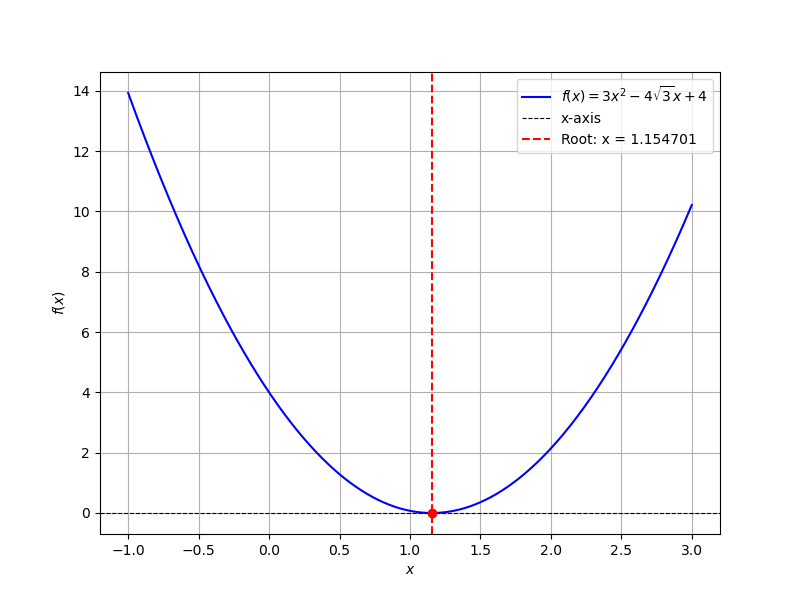
\includegraphics[width=0.75\columnwidth]{figs/eq.png}
\end{center}

\end{document}